\documentclass[12pt, titlepage]{article}

\usepackage{booktabs}
\usepackage{tabularx}
\usepackage{hyperref}
\usepackage{float}
\usepackage{graphicx}
\usepackage[normalem]{ulem}
\usepackage{xcolor}
\hypersetup{
    colorlinks,
    citecolor=black,
    filecolor=black,
    linkcolor=red,
    urlcolor=blue
}
\usepackage[round]{natbib}

\title{SE 3XA3: Software Requirements Specification\\Mastermind}

\author{Team 204, Trident Inc.
		\\ Justin Rosner, rosnej1 
		\\ Justin Prez, prezj
		\\ Harshil Modi, modih1
}

\date{\today}

%\input{../Comments}

\begin{document}

\maketitle

\pagenumbering{roman}
\tableofcontents
\listoftables
\listoffigures

\begin{table}[hp]
\caption{Revision History} \label{TblRevisionHistory}
\begin{tabularx}{\textwidth}{llX}
\toprule
\textbf{Date} & \textbf{Developer(s)} & \textbf{Change}\\
\midrule
2020-01-22 & Justin Rosner, Justin Prez, Harshil Modi & Initial write-up of SRS document\\
\textcolor{red}{2020-04-04} & \textcolor{red}{Justin Rosner, Justin Prez, Harshil Modi} & \textcolor{red}{Revision 1 of SRS}\\
\bottomrule
\end{tabularx}
\end{table}


\newpage

\pagenumbering{arabic}

\section{Project Drivers}

\subsection{The Purpose of the Project}
The purpose of this project is to recreate the famous 1970s game Mastermind with a user-friendly graphic user interface (GUI), and additional levels of difficulty to captivate the user. After the initial hype of the game in the 1970s, the number of users that play the game has decreased drastically. With the new and improved design, our team aims to make Mastermind a game that is played and enjoyed by everyone once again.

\subsection{The Stakeholders}

\subsubsection{The Client}
The clients of our project are \sout{academia/professional psychologists and the final commissioners that will be making profit of the deployment of the app. Academia and professional psychologists will use the new and improved game as part of the IQ test instead of the older version. Additionally, final commissioners include researchers interested in the link between mastermind and IQ.} \textcolor{red}{the TA's of SFWRENG 3XA3, and Professor Bokhari as they are commissionin the project}

\subsubsection{The Customers}
In this case the customers \textcolor{red}{are the} \sout{include the clients plus the} end users of the product. The end user includes individuals of all ages over the MIN\_AGE and can obtain a computer/tablet. Mastermind will be free to obtain by anyone through the Google play store or Apple app store.

\subsubsection{Other Stakeholders}
Additional \sout{stakeholder} \textcolor{red}{stakeholders} of the product include McMaster university, the development team consisting of Harshil Modi, Justin Prez, Justin Rosner, \textcolor{red}{as well as academia/professional psychologists and the final commissonsers that will be making profit off of the development of the app. Academia and professional psychologists will use the new and improved game as part of an IQ test instead of the older version of the game. Furthermore, final commissioners include researchers interested in the link between Mastermind and IQ.}

\subsection{Mandated Constraints}

\subsubsection{Solution Constraints}
\begin{itemize}
\item \textbf{Description:} The product shall be operational on both iOS and Android devices.\\
\textbf{Rationale:} iOS and Android are the main operating systems used by our customers and clients.
\item \textbf{Description:} The app should be downloadable through the Apple app store and Google play store.
 \\
\textbf{Rationale:} Customers and clients will have Android or iOS devices.

\item \textbf{Fit Criterion:} The product should be compatible with both mobile and tablet devices of varying size.\\
\textbf{Rationale:} Clients will be using our app on both mobile and tablet with different screen sizes.
\end{itemize}
\subsubsection{Implementation Environment of the Current System}
\sout{N/A} \textcolor{red}{The technological environment in which the product is to be installed is the iOS operating system for Apple products and the Android operating system for Android devices.}

\subsubsection{Partner or Collaborative Application}
To run the software on a computer, the user will require the Flame library for game implementation. The software will not be expected to run if Flame is not installed on the User’s computer. 

For users who download the app on their smart device, no such installation is required.
 
\subsubsection{Off-the-Shelf Software}

\begin{itemize}
    \item \textbf{Description:} The design will utilize the Flame library for game development.\\
\textbf{Rationale:} Flame is a very famous game building library in Flutter and due to limitations in time and resources there is no need to reinvent the wheel.
\item \textbf{Description:} The design will make use of the Flutter framework for the UI\\
\textbf{Rationale:} Flutter is a well documented framework that will make development of the UI much easier.
\end{itemize}

\subsubsection{Anticipated workplace Environment}
The anticipated workplace environment for Mastermind is everywhere. It is intended to be played in the house, on-the-go, public places etc. The application does not require access to mobile data or the internet hence it is accessible to all clients.

\subsubsection{Schedule constraints}
\begin{itemize}
    \item \sout{There are no set schedule constraints for our application however the documentation of the software will be delivered by the deadlines specified in the SE3XA3 outline.} \textcolor{red}{The Proof of Concept Demonstration for Revision 0 is due week of February 14 2020}
    \item \textcolor{red}{The Test Plan for Revision 0 is due February 28 2020}
    \item \textcolor{red}{The Design \& Documentation documents for Revision 0 are due March 13 2020}
    \item \textcolor{red}{The Revision 0 demonstration is the week of March 16 2020}
    \item \textcolor{red}{The Final Demonstration for Revision 1 is the week of March 30 2020}
    \item \textcolor{red}{The Final Documentation for the project is due April 6 2020}
    \item \sout{The unofficial deadline for mastermind’s final implementation is set to April 1st  2020.}
\end{itemize}

\subsubsection{Budget constraint}
Budget constraint is not applicable here as all the resources needed to complete the game have been provided to us.


\subsection{Naming Conventions and Terminology}
\begin{itemize}
    \item \textbf{GUI:} graphical User Interface, the interface that the user interacts with that includes graphical elements, icons, and buttons.
    \item \textbf{Mastermind:} A two person game with pegs invented by Mordecia Meirowitz.
    \item \textbf{Flame:} A minimalist Flutter game engine library for creating easy to build games.
    \item \textbf{FPS:} Frames per second. A tool to measure the refresh speed of a image.
    \item \textbf{Dart:} A client optimized language for fast multi-platform app development.
    \item \textbf{Flutter:} Google’s UI toolkit for crafting natively compiled applications for mobile development. 
    \item \textbf{UI:} The interface which the user sees and interacts with. Similar to the GUI in this case.
    \item \textcolor{red}{\textbf{Pegs:} What the user will see in an empty spot on the game board after making a guess. Pegs can be Red, Blue, Green, Yellow, White, Purple.}
    \item \textcolor{red}{\textbf{Hints:} Small tiles beside teh game board that will tell the user how many of their guesses are in the correct position and are the correct colour.}
    \item \textcolor{red}{\textbf{Correct Guess:} This is the correct sequence of pegs that the user will need to input in order to win}

\end{itemize}

\subsection{Relevant Facts and Assumptions}
\subsubsection{Relevant Facts}
\begin{itemize}
    \item Flame is capable of hosting and running mastermind style games.
    \item Dart and Flutter are proven to be capable of running mobile games on both iOS and android.
    \item The original project has less than 700 lines of code in python.
    \item Mastermind is known to be one of the tools to determine a person's IQ.
\end{itemize}
\subsubsection{Relevant Assumptions}
The target user of the product is assumed to be:

\begin{itemize}
    \item Mentally competent to play mastermind
    \item Physically capable of touching the screen with hand-eye coordination
    \item Interested in IQ evaluation methods
\end{itemize}

The average user will have :

\begin{itemize}
    \item A relatively modern phone or tablet capable of running mastermind.
    \item Access to the Google Play Store or Apple App Store, as well as to the internet to download the game.
\end{itemize}

\sout{User characteristics should go under assumptions.}

\section{Functional Requirements}

\subsection{The Scope of the Work and the Product}
\subsubsection{The Context of the Work}
\begin{figure}[H]
   \centering
   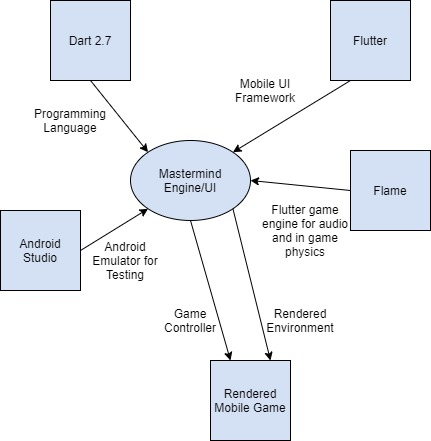
\includegraphics[scale=0.5]{context_of_work.jpg}
   \caption{Context of the Work.}
   \label{fig:context_of_work}
 \end{figure}
 
\subsubsection{Work Partitioning}
\begin{table}[H]
\caption{Work Partitioning}
\begin{tabular}{@{}lll@{}}
\toprule
\textbf{Event Name}       & \textbf{Input and Output} & \textbf{Summary}  \\ \midrule
1. Mastermind Game Creation & Developer code (in) &  \begin{tabular}[c]{@{}l@{}}Recreate mastermind game \\ logic in Dart with same \\logic as original code base.\end{tabular} \\ \midrule
2. Mastermind Additional Level & Developer code (in) & \begin{tabular}[c]{@{}l@{}}Add additional challenges\\ to the original mastermind\\ game.\end{tabular} \\ \midrule
3. Player makes a guess  & \begin{tabular}[c]{@{}l@{}} Player guess (in) \\ Show correct guesses (out)\end{tabular}  & \begin{tabular}[c]{@{}l@{}} Update the state of \\ board and allow user \\ option to make more \\ guesses \end{tabular} \\ \midrule
4. Game finishes & \begin{tabular}[c]{@{}l@{}}Final Player Guess(in) \\ End of game message(out)\end{tabular} & \begin{tabular}[c]{@{}l@{}}Update state of board to \\  finished.\end{tabular} \\ \bottomrule
\end{tabular}
\end{table}

\subsubsection{Individual Product Use Cases}
The main use case\textcolor{red}{s} for this product allow\sout{s} for users to start a new game, make guesses, and view the rules of the game. \sout{This case is} \textcolor{red}{These cases are} outlined in the diagram below.  

\begin{figure}[H]
   \centering
   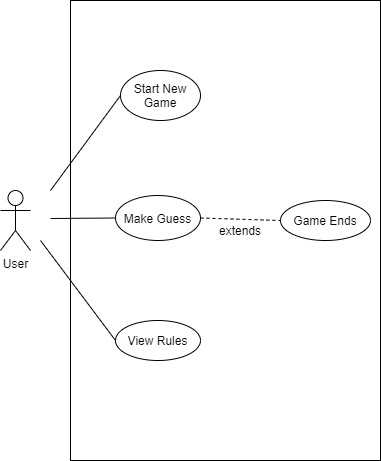
\includegraphics[scale=0.5]{use_cases.jpg}
   \caption{Use Case Diagram.}
   \label{fig:use_case}
 \end{figure}

\subsection{Functional Requirements}
\begin{itemize}
    \item \textbf{REQ1:} The game will be implemented using Dart and Flame library.
    \item \textbf{REQ2:} The user must be able to select  a blue colour peg using the touch screen.
    \item \textbf{REQ3:} The user must be able to select  a yellow colour peg using the touch screen.
    \item \textbf{REQ4:} The user must be able to select  a red colour peg using the touch screen.
    \item \textbf{REQ5:} The user must be able to select  a green colour peg using the touch screen.
    \item \textbf{REQ6:} The user must be able to select  a white colour peg using the touch screen.
    \item \textbf{REQ7:} The user must be able to select  a purple colour peg using the touch screen.
    \item \textbf{REQ8:} The user must be able to place the pegs onto the board using the touch screen.
    \item \textbf{REQ9:} \sout{The user must be able to view the help screen using the touch screen.}
    \textcolor{red}{The user must be able to view the instructions on how to play the game upon opening up the application.}
    \item \textbf{REQ10:} The user must be able to close the game using the touch screen.
    \item \textcolor{red}{\textbf{REQ11:} The user shall be able to select 4 pegs as a guess.}
    \item \textcolor{red}{\textbf{REQ12:} The system shall display hints to the user after each guess.}
    \item \textcolor{red}{\textbf{REQ13:} The correct sequence of pegs shall be displayed to the user after 10 incorrect guesses.}
    \item \textcolor{red}{\textbf{REQ14:} The user shall be able to undo a peg press if the row (guess) is not complete.}

\end{itemize}

\section{Non-Functional Requirements}
\subsection{Look and Feel Requirements}
\subsubsection{Appearance}
\begin{itemize}
\item \textbf{LF1:} GUI should be visually appealing to users of our market audience. The colours representing buttons or game features should be easily distinguishable, and not blend with the background colour.\\
\textbf{Fit Criterion:} After the initial release of the project a survey should be completed by users to show that 95\% of users enjoyed using the product.
\end{itemize}

\subsubsection{Style}
\begin{itemize}
\item \textbf{LF2}: The GUI should resemble the classic board from the game of Mastermind.\\
\textbf{Fit Criterion:} After the initial release of the project a survey should be completed by users to show that 95\% of users thought the product resembled the classical version of Mastermind.
\end{itemize}

\subsection{Usability and Humanity Requirements}

\subsubsection{Ease of Use Requirements}
\begin{itemize}
\item \textbf{UH1}: The game shall be playable by people MIN\_AGE and up.\\
\textbf{Fit Criterion:} A sample study of users MIN\_AGE and up interacting with the game should show that 90\% of them were able to play the game properly without additional assistance.
\item \textbf{UH2}: The user shall be able to easily download and play the game on their smart device.\\
\textbf{Fit Criterion:} Testing will be done to ensure that there are no issues downloading the game from the Google Play Store or Apple App Store.
\item \textbf{UH3}: The application shall be engaging and fun for users to play.\\
\textbf{Fit Criterion:} \textcolor{red}{Four months after} \sout{After} the release of the product, \sout{the ratings on the Google Play Store and Apple App Store should be above 4 (out of 5)} \textcolor{red}{a sample of users will be asked to play the game, and after the experience 90\% of the users should have said that they had fun and\/or engaging.}.
\end{itemize}


\subsubsection{ Personalization and Internationalization Requirements}
\begin{itemize}
    \item \textbf{UH5}: The product shall allow users to select their preferred language.\\
    \textbf{Fit Criterion:} A software test engineer will make sure that the users have the option to select their preferred language.
\end{itemize}

\subsubsection{Learning Requirements}
\begin{itemize}
    \item \textbf{UH6}: Users of MIN\_AGE and up shall be able to play the game with no prior experience or training.\\
    \textbf{Fit Criterion:} A sample of users will be asked to play the game with no instructions. After PLAY\_TIME minutes 90\% of the users would have figured out how.
    \item \textbf{UH7}: Users shall be able to remember how to play the game after their first experience.\\
    \textbf{Fit Criterion:} The same sample of users used in the criterion above will be asked back a week after their first session to test for memory retention. 95\% of said users should have remembered how to play the game. 
    \item \textbf{UH8}: Instructions shall be provided for the rules of the game.\\
    \textbf{Fit Criterion:} N/A

\end{itemize}

\subsubsection{Accessibility Requirements}
\begin{itemize}
\item \textbf{UH9}: The product shall use symbols and words that are naturally understandable by users. \\
\textbf{Fit Criterion:} Users will be invited in for an in-person assessment of symbols and words used in Mastermind. 95\% of said symbols and words have to be deemed understandable by the group of users. 
\item \textbf{UH10}: Language used to describe the rules shall be easy to understand with no grammar or spelling errors.\\
\textbf{Fit Criterion:} A software test engineer will test to make sure that there are 0 spelling or grammatical errors in the application.
\item \textbf{UH11}: The implementation of the product shall be hidden from the users.\\
\textbf{Fit Criterion:} Users should not be able to access or view any of the source code from within the app.
\end{itemize}


\subsection{Performance Requirements}
\subsubsection{Speed and Latency Requirements}
\begin{itemize}
\item \textbf{PR1}: The game interface shall respond to user input in under MIN\_RESPONSE\_TIME.\\
\textbf{Fit Criterion:} A software test engineer will perform a series of \textcolor{red}{NUM\_STRESS\_TESTS} \sout{100} stress tests to ensure that response time is always under MIN\_RESPONSE\_TIME. \textcolor{red}{NUM\_STRESS\_TESTS divided by NUM\_STRESS\_TESTS}\sout{100/100} of the test cases shall pass.
\end{itemize}

\subsubsection{Safety-Critical Requirements}
\begin{itemize}
\item \textbf{PR2}: The product will not encourage violence, discrimination or cause addictive behaviour. \\
\textbf{Fit Criterion:} A survey will be conducted after the release of the product asking users if they have experienced an increase in any of the aforementioned behaviours since starting to use the app. 98\% of the users shall not have experienced any of the negative behaviours.
\end{itemize}

\subsubsection{Precision or Accuracy Requirements}
\begin{itemize}
\item \textbf{PR3}: User input shall translate directly to the intended output within the context of the game.\\
\textbf{Fit Criterion:} A software test engineer will perform \sout{200} \textcolor{red}{NUM\_TEST\_CASES} test cases where the intended output is generated from the input 100\% of the time.
\item \textbf{PR4}: All colors displayed on the GUI shall be easily distinguishable.\\
\textbf{Fit Criterion:} A survey will be conducted on users asking about distinguish-ability of colours, 95\% of users shall say that the colours were distinguishable.
\end{itemize}

\subsubsection{Reliability and Availability Requirements}
\begin{itemize}
\item \textbf{PR5}: The product shall be available for use UP\_TIME.\\
\textbf{Fit Criterion:} The system will be tested once a day to ensure that there are no problems.
\item \textbf{PR6}: The product shall achieve this UP\_TIME, by using previous stable versions of the game for users during product maintenance.\\
\textbf{Fit Criterion:} \sout{N/A} \textcolor{red}{Throughout testing, a software test engineer will check in on the state of the game periodically throughout the game to make sure that it never goes down.}
\end{itemize}

\subsubsection{Robustness or Fault-Tolerance Requirements}
\begin{itemize}
\item \textbf{PR7}: The product shall be playable without internet connection.\\
\textbf{Fit Criterion:} A software test engineer will play \sout{100} \textcolor{red}{MIN\_NUM\_TESTS} iterations of the game with their device disconnected from the internet. They shall be able to successfully play 100\% of the time.
\end{itemize}

\subsubsection{Capacity Requirements}
\begin{itemize}
\item \textbf{PR8}: The product shall be able to handle the loading of an individual user.\\
\textbf{Fit Criterion:} A software test engineer will play \sout{100} \textcolor{red}{MIN\_NUM\_TESTS} iterations of the game, with 100\% success rate for completion of the game.
\end{itemize}

\subsubsection{Scalability or Extensibility Requirements}
\begin{itemize}
\item \textbf{PR9}: The product shall be implemented to allow for easy modification and improvement.
\item \textbf{PR10}: The product shall allow for the implementation of new features.\\
\textbf{Fit Criterion:} The modularity of the software design will be verified by a third-party, by having them attempt to modify or add a feature to the game.
\end{itemize}

\subsubsection{Longevity Requirements}
\begin{itemize}
\item \textbf{PR11}: The product shall be expected to operate on all smart devices for the next several iOS and android system updates.\\
\textbf{Fit Criterion:} After the next major iOS or Android update, a survey will be given to users to gauge if their ability to play was impacted in anyway. 
\end{itemize}

\subsection{Operational and Environmental Requirements}


\subsubsection{Expected Physical Requirements}
\begin{itemize}
\item \textbf{OE1}: The product shall be usable in any physical environment that a user can view their phone.\\
\textbf{Fit Criterion:} The project should be able to run any smart device with iOS or Android, or any computer with Flame downloaded.
\end{itemize}

\subsubsection{Requirements for Interfacing with Adjacent Systems}
\begin{itemize}
\item \textbf{OE2}: The product shall run on all smart devices running iOS or android operating systems. \\
\textbf{Fit Criterion:} Our application will be tested to run on several different devices to ensure compatibility.
\item \textbf{OE3}: The product shall run using the most recent version of Dart (Dart 2.7).\\
Fit Criterion: N/A
\end{itemize}

\subsubsection{Productization Requirements}
\begin{itemize}
    \item \textbf{OE4}: The product shall be able to be installed by an untrained user.\\
    \textbf{Fit Criterion:} The product will be available on trusted platforms like the Apple app store or   Google play store, where users have experience downloading trusted applications for their smart device. 
\end{itemize}

\subsubsection{Release Requirements}
\begin{itemize}
    \item \textbf{OE5}: The maintenance releases will not cause previous features to fail.\\
    \textbf{Fit Criterion:} Maintenance releases will be thoroughly tested before release to ensure that all current working features are not impacted by new fixes/changes. 
    
\end{itemize}

\subsection{Maintainability and Support Requirements}

\subsubsection{Maintenance Requirements}
\begin{itemize}
    \item \textbf{MS1}: The product shall be updated when new bugs or glitches are known.\\
    \textbf{Fit Criterion:} The developers will release a new patch every month to fix any bugs that have been made known by the community, or to release new content and features for the game.
    
    \item \textbf{MS2}: Maintenance releases shall be accompanied by patch updates to notify users of changes, new features or fixes.\\
    \textbf{Fit Criterion:} N/A
    
\end{itemize}

\subsubsection{Support Requirements}
\begin{itemize}
    \item \textbf{MS3}: Other programmers shall be allowed to identify and fix bugs for the open source product.\\
    \textbf{Fit Criterion:} Contributions from other programmers will be validated before committing changes to the project.
\end{itemize}

\subsection{Security Requirements}
\subsubsection{Access Requirements}
\begin{itemize}
    \item \textbf{SR1}: The product software will be free to download.\\
    \textbf{Fit Criterion:} N/A
\end{itemize}

\subsubsection{Integrity Requirements}
\begin{itemize}
    \item \textbf{SR2}: All data is stored on the user’s local machine.\\
    \textbf{Fit Criterion:} N/A
    
    
    \item \textbf{SR3}: The product shall protect itself from intentional abuse such as cheating.\\
    \textbf{Fit Criterion:} Thorough testing will ensure that 99\% of the data introduced to the game is safe from tampering that would allow players to cheat.
    
\end{itemize}

\subsubsection{Privacy Requirements}
\begin{itemize}
    \item \textbf{SR4}: The product will not collect or store any user data.\\
    \textbf{Fit Criterion:} The develops will not retain a single instance of personal information from users.
\end{itemize}

\subsubsection{Audit Requirements}
\begin{itemize}
    \item N/A
\end{itemize}

\subsubsection{Immunity Requirements}
\begin{itemize}
    \item \textbf{SR5}: All product download links shall be cleared of malicious software and viruses.\\
    \textbf{Fit Criterion:} All download links issued by the development team will be thoroughly tested and secured to guarantee safe downloads.
    
    \item \textbf{SR6}: The product shall be installed only using trusted sources. \\
    \textbf{Fit Criterion:} Provide a disclaimer to state that we are not responsible for download links not provided by our team.
\end{itemize}

\subsection{Cultural and Political Requirements}
\begin{itemize}
    \item \textbf{CP1}: The product shall not discriminate any racial, political, cultural, or ethnic group.\\
    \textbf{Fit Criterion:} Several months after the product release, a community poll will be conducted to gather feedback from the user community on any controversial subjects that they want to address.
\end{itemize}
\subsection{Legal Requirements}
\begin{itemize}
    \item \textbf{LE1}: The product shall not violate any copyright or intellectual property laws.\\
    \textbf{Fit Criterion:} Lawyers will review the product to ensure that the game does not violate any laws of copyright or stolen intellectual property.
\end{itemize}
\subsection{Health and Safety Requirements}
\begin{itemize}
    \item \textbf{HS1}: The product shall not endanger or harm the user.\\
    \textbf{Fit Criterion:} A test team will perform a risk analysis of the product to validate that it is safe for all users.
\end{itemize}

\section{Project Issues}

\subsection{Open Issues}
N/A
\subsection{Off-the-Shelf Solutions}
There currently exists many other free versions of Mastermind similar to the existing implementation. The common theme among all of these versions is that the graphical user interface is lacking in quality, and this is what our group aims to improve on.

These free versions can be used as a template to create the main logic for the basic version of the game. The benefit of using these other versions as templates is that it allows for our group to see where the current inefficiencies and trouble areas are, and work to fix these to improve the project.

Furthermore, there are many online resources for using Dart and Flutter to create 2-D games that our group will be able to utilize.
\subsection{New Problems}
\subsubsection{Effects on the Current Environment}
\sout{N/A} \textcolor{red}{The application should not take or use any data from the device that it is being played on. Furthermore, the application shall not alter or leave behind any malicious software on the device.}
\subsubsection{Effects on the Installed Systems}
N/A
\subsubsection{Potential User Problems}
Any prolonged exposure to screens due to playing of Mastermind may potentially have adverse effects on the user's eyesight and eyes as a whole.
\subsubsection{Limitations in the Anticipated Implementation Environment That May Inhibit the New Product}
The development team has minimal experience making games using Dart and Flutter, so this may cause some issues when implementing some of the fine grain details of the user interface. The development team should focus on creating a simple and aesthetic version of the game first, before they decide to add some of the more intricate GUI details.
\subsubsection{Follow-Up Problems}
If there are updates to the Android operating system, the Dart/Flutter app may no longer be compatible. In this case maintenance would have to be done to ensure compatibility with the operating system.

\subsection{Tasks}
\subsubsection{Project Planning/Development Process}
Please refer to the \href{https://gitlab.cas.mcmaster.ca/rosnej1/open-mastermind/-/blob/master/ProjectSchedule/ProjectSchedule.pdf}{ProjectSchedule/ProjectSchedule.pdf} in the repository for a Gantt Chart detailing the tasks required for this project.

\subsection{Migration to the New Product}
\subsubsection{Requirements for Migration to the New Product}
N/A
\subsubsection{Data That Has to be Modified or Translated For the New System}
N/A

\subsection{Risks}
\subsubsection{Excessive Schedule Pressure}
Should the development team have any issues learning how to use Dart and Flutter then there is the potential to fall behind schedule as it would be very difficult to meet deadlines as well as learning the language/framework.
\subsubsection{Management Malpractice}
The development team will have to follow the plan outlined in the Gantt chart and ensure that proper use of time and resources is allocated in order to complete the project by the required due dates. 
\subsubsection{Low Quality}
When developing games there is always the possibility of the team becoming too ambitious and focusing on the finer grained details rather than getting the main logic of the game working smoothly. This would result in a low quality game, thus letting the stakeholders down. To combat this risk the development team should focus on getting a basic implementation of the game working before any additional features are attempted

\subsection{Costs}
The developers will be making use of the open source languages; Dart and Flutter to create the product. Therefore there will be no costs associated with the development process.

\subsection{User Documentation and Training}
\subsubsection{User Documentation Requirements}
The development team will provide the user with an option to view the rules of the game from the start menu. The rules will dictate to the user how the game is to be played. Furthermore, inside of the game if a user makes an illegal move, the game will prohibit it and provide an explanation to the user on why the move was not allowed.
\subsubsection{Training}
There is no training required to use the product.

\subsection{Waiting Room}
At this time \sout{there is no plan to create additional functionality not already mentioned in the requirements.} \textcolor{red}{some of the ideas that the team has for future additions to the game are: }
\begin{itemize}
    \item \textcolor{red}{Adding varying levels of difficulty to the game. Currently the game requires the user to correctly guess a combination of 4 pegs, we could instead add an easier difficulty where they only have to guess 3 pegs, and likewise a more difficult setting where they have to try and guess 5 pegs.}
    \item \textcolor{red}{Adding support for multiple languages (French, Spanish, etc.)}
    \item \textcolor{red}{Create a desktop version of the application.}
    \item \textcolor{red}{Create a "Play a Friend" mode in which two friends will be able to play MasterMind over a server.}
    \item \textcolor{red}{Create a leader board in which the user will be able to see their all time win percentage, as well as their friends statistics.}
\end{itemize}

\subsection{Ideas for Solutions}
The team plans to user proper documentation, code hierarchy, and testing. Alternatively, the team could use a different combination of languages/graphics libraries such as python and pygame for the implementation.

\newpage

\section{Appendix}


\subsection{Symbolic Parameters}

The following are definitions of symbolic constants that are used throughout this document:

\begin{itemize}
    \item MIN\_AGE: 4
    \item MIN\_RESPONSE\_TIME: 0.5 Seconds
    \item UP\_TIME: 24 hours a day, 365 days a year
    \item \textcolor{red}{PLAY\_TIME: 10 Minutes}
    \item \textcolor{red}{NUM\_STRESS\_TEST: 100}
    \item \textcolor{red}{NUM\_TEST\_CASES: 200}
    \item \textcolor{red}{MIN\_NUM\_TESTS: 100}
    
    
\end{itemize}



\end{document}
